%BALLISTIC PENDULUM
\newexp

\section*{Before Lab}

Please read this writeup carefully, and be sure you can derive
Equations (\ref{v(y)}) and (\ref{y(xL)}).  Work out these
derivations in your lab notebook.  Your TA will check them at the
beginning of the lab period.  It may also be helpful to review the
concepts of standard deviation and standard deviation of the mean.

\section*{Introduction}

In a collision the total momentum of the colliding bodies is
unchanged---that is, momentum is conserved---if the net external force is
zero.  However,
mechanical energy may or may not be conserved.  In the study of
collisions, two extremes are generally
defined.  A {\em perfectly elastic} collision is one in which the
total kinetic energy of the system doesn't change.  Collisions of
microscopic objects such as atoms, for example, often fit into this
category.  If the kinetic energy is changed following the collision, 
the collision is inelastic.  A {\em perfectly
inelastic} collision is one in which the colliding objects stick
together.  In this experiment we will use a device known as a
ballistic pendulum to study inelastic collisions and to measure the
velocity of a projectile.

%You will also get practice with some basic
%statistical analysis techniques.

\section*{Apparatus}
\be
\item Projectile launcher, steel ball;
\item Ball catcher suspended from an aluminum rod;
\item Steel rail with tinfoil marker;
\item Tape measure and scale (somewhere in the lab);
\item Plumb line;
\item Meter stick.
\ee
\section*{Experiment}

In this experiment we will be shooting a steel ball horizontally from
a launcher, as illustrated in Fig.~\ref{bpend}.  The ball will be
caught by a cylindrical container suspended as a pendulum from strings
mounted on an aluminum rod.  By measuring the horizontal distance the
pendulum swings we can calculate the ball's initial velocity $v$.

We will compare this result with the velocity calculated by shooting
the projectile horizontally and measuring how far it travels.

%With this information you should also be able
%to determine how far the launcher can shoot the ball.

%\newpage
%\vspace*{2in}
\bfig[h]
\begin{center}
{\resizebox{5.5in}{!}{{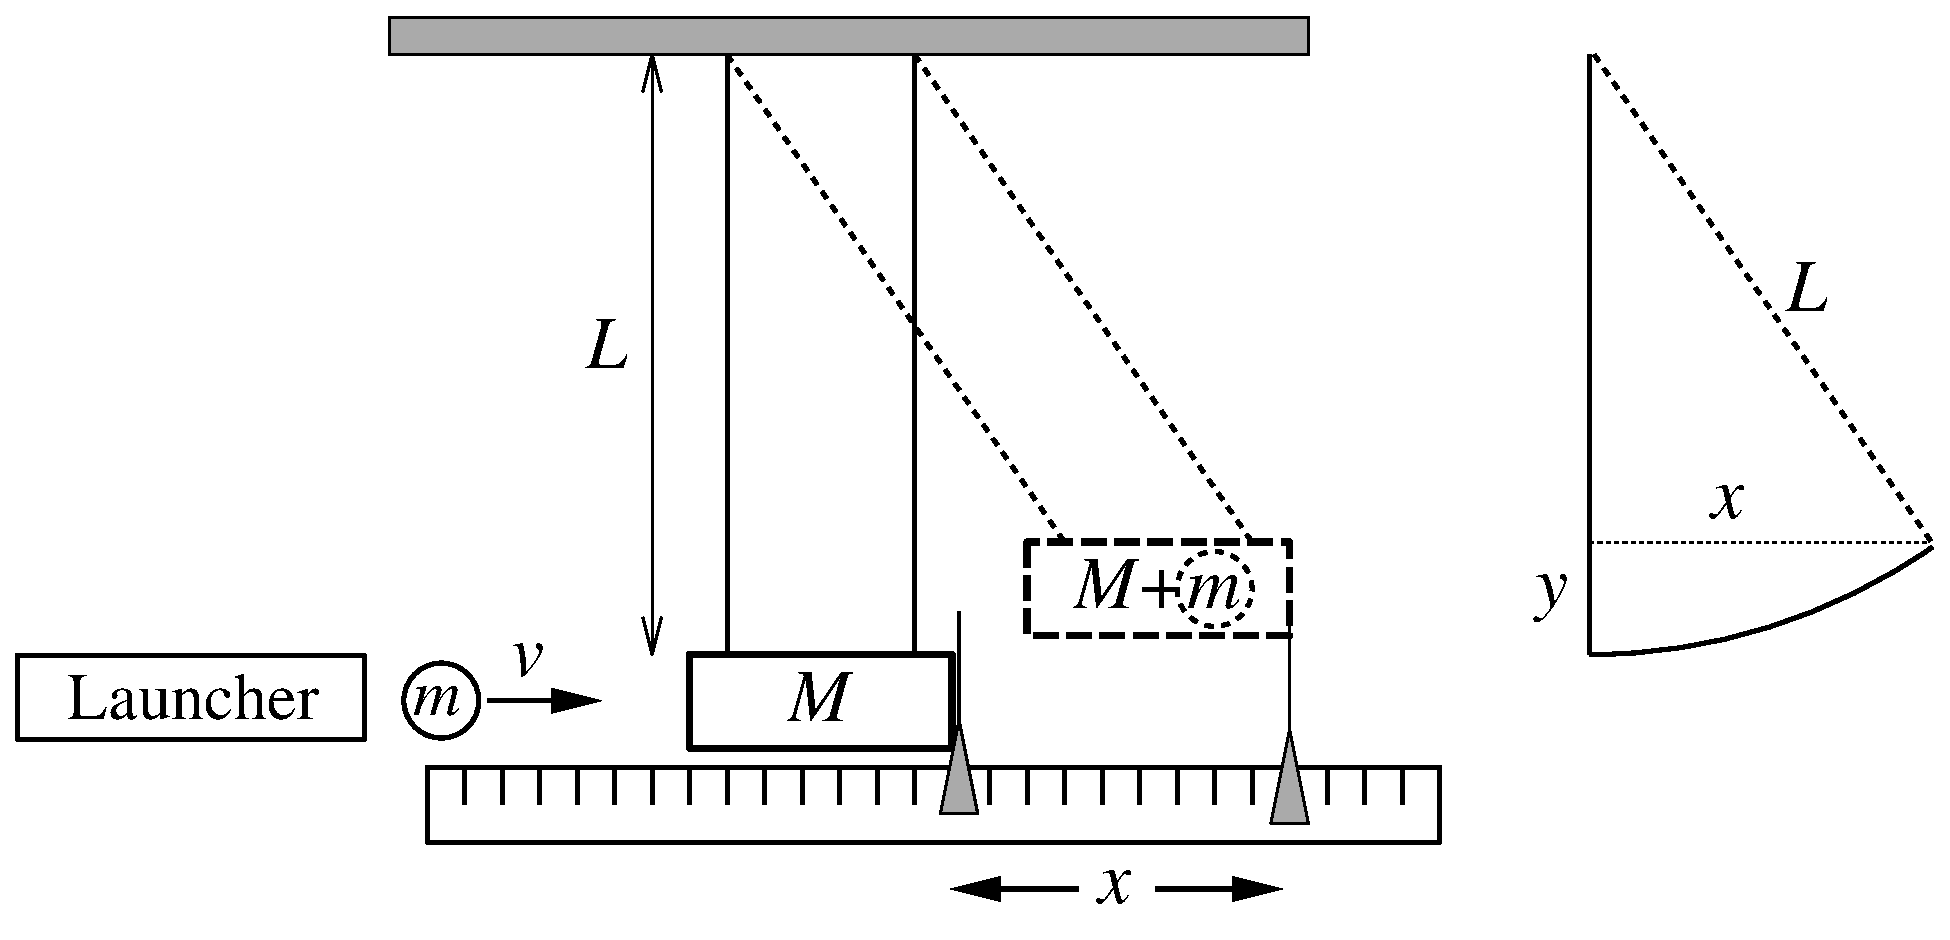
\includegraphics{ballis2.eps}}}}
\end{center}
%\special{eps:\location ballis1.eps x=5.5in y=2in}
%\special{eps:ballis1.eps x=5.5in y=2in}
\caption{Ballistic pendulum experiment. \label{bpend}}
\efig

\section*{Theory}

Consider Fig.~\ref{bpend} above:  We launch a
spherical steel projectile
at a cylindrical ``catcher.''  The two collide and stick together, and
thereafter move as one.  It is convenient to divide this process
conceptually into two parts.

First part: During the collision itself, momentum is conserved, but
energy is not, since the collision is inelastic.  Thus, the momentum
$p_{i}$ before the collision equals $p_{f}$, the momentum after the
collision.  In equation form,

\beq
p_{i} = mv = p_{f} = (m+M)V, \label{pi=pf}
\eeq

where $m$ is the ball's mass, $M$ is the catcher mass, $v$ is the
ball's initial velocity and $V$ is the velocity of the catcher and
ball immediately after the collision.

Second part:  Immediately after the collision, the ball/catcher system
becomes the bob of a pendulum that moves off at some initial velocity
$V$, as shown in Eq.(\ref{pi=pf}) above. The pendulum's initial
kinetic energy changes to gravitational
potential energy as it swings and rises to a height $y$, where it is
instantaneously at rest. Momentum is clearly not
conserved in this second part of the experiment as the
pendulum slows, stops, and reverses. The motion
of the system is nearly frictionless, so mechanical energy {\it is} nearly
conserved for this part of the motion.  We express this conservation
law in the equation

\beq
\frac{1}{2}(m+M)V^{2} = (m+M)gy. \label{KE=PE}
\eeq

If we combine Eqs.~(\ref{pi=pf})~and~(\ref{KE=PE}), it is easy to
show that the initial velocity of the projectile is related to the
height $y$:

\beq
v = \left(1+\frac{M}{m}\right)\sqrt{2gy}. \label{v(y)}
\eeq

It would be difficult to measure the change in height $y$ directly.
Instead, we will measure the horizontal distance $x$ that the pendulum
moves, and use this quantity to calculate $y$.  If we consider
Fig.~\ref{bpend}, it is clear the the string length $L$ is
the hypotenuse of a right triangle with sides $(L-y)$ and $x$, so:

%\beq
%L^{2} = x^{2} + (L-y)^{2} = L^{2} + x^{2} + y^{2} - 2Ly, \label{quad}
%\eeq
%which is a quadratic equation for $y$ with the solutions
%\beq
%y = L \pm \sqrt{L^{2}-x^{2}}. \label{y(xL)}
%\eeq
%The minus sign gives the solution which is relevant here.  (Can you
%explain what the other one means?) So by measuring $x$, the initial
%velocity $v$ of the ball can be calculated.

\beq
L^2 = (L-y)^2 + x^2
\eeq

If we subtract $x^2$ from both sides we obtain

\beq
L^2 - x^2 = (L-y)^2.
\eeq

If we now take the (positive) square root and solve for $y$,
we find

\beq
y = L - \sqrt{L^{2}-x^{2}}. \label{y(xL)}
\eeq

We will use this expression for $y$ in Eq.~(\ref{v(y)}) above to
calculate $v$.

We also want to find the uncertainty in the initial projectile
velocity $v$.  The measured quantities, $x$, $L$, $m$, and $M$ all
have some uncertainty, leading to uncertainty in the calculated $v$.
The formulas connecting $v$ with these measured quantities would make
the error analysis complicated.  In addition, another source of
uncertainty is in the behavior of the launcher---one sometimes sees
variations in $v$ from shot to shot.

Under these circumstances, a good way to estimate 
uncertainty is repeated measurement.
%both the velocity
%and the uncertainty in the velocity is to fire the ball repeatedly,
%and calculate the mean velocity and the standard deviation of the mean
%as an estimate for the uncertainty.  
Suggestions for a detailed
procedure are given below.

%Finally, we can calculate the change in kinetic energy.  Kinetic
%energy will be lost in any non-elastic collision. In the {\em
%perfectly} inelastic case, one can readily show from Eq.~(\ref{pi=pf})
%that
%
%\beq
%\frac{KE_{{\rm before}}}{KE_{{\rm after}}} =
%\frac{\frac{1}{2}mv^{2}}{\frac{1}{2}(m+M)V^{2}} = \frac{m+M}{m}
%\label{KEratio}
%\eeq



\section*{Procedure and Data Analysis}

\be

%\item BEFORE YOU COME TO LAB: Do the algebra to obtain
%Eqs.~(\ref{v(y)}), (\ref{y(xL)}), and (\ref{KEratio}).  Be ready to
%show all this to your TA, or to deal with these concepts on a quiz.

%\item

\item Use the digital balance to measure the masses $m$ and $M$ of the
ball and catcher.  (The mass of the catcher may already be given.) 
Use the tape measure to measure the string length
$L$, {\it after} you have completed the alignment procedure described
below. Record these values in your notebook.

\item  Alignment Procedure for the Ballistic Pendulum

Identify the projectile launcher, the catcher, and the foil slider.
Be sure that the launcher on your table is mounted so that it shoots
horizontally.  Be sure that it positioned close to the catcher.

It is {\bf important} that the projectile launcher, catcher, and foil
slider all be aligned along the same axis.  Each must also be
level.  Take your time, and be sure follow this procedure carefully.

	\begin{itemize}

	\item  To align along the same axis, place the slider track
	under the catcher and clamp the launcher in place.  Looking
         down the slider track, all three should appear to line up.
	
	\item The height of the catcher can be adjusted by raising or
	lowering the vertical rod holding the catcher in place. 
       The string support 
        can be leveled by loosening the support clamp and rotating the
        topmost support assembly.  The
	catcher should barely clear ($\sim 1/8"$) the slider
	track.  The catcher should also be at the same level as the
	launcher.
	
	\item The launcher can be leveled by loosening a wing nut
and rotating it.
	The catcher can be leveled
        by pulling string through the catcher.  
	
	\end{itemize}


\item Loading the Launcher

	\begin{itemize}

	\item The ball should be inserted into the launcher with the
        wooden dowel.  Always listen for the same number of clicks.
        (We have had the best luck using three clicks; but feel free
        to experiment.)

	\item  Use the same wooden dowel to remove the ball from the
        catcher.  To accomplish this, pull the catcher to one side of
        the track and push the dowel into the far end of the catcher.
	
	\item Notice that there are three settings for the launch
        velocity --- you can try them all to decide which one you
        want.  Take some practice shots to make sure everything works
        correctly.  Make sure the tinfoil marker slides with hardly
        any resistance on the rail.  Make sure the catcher swings
        upward without rotating.  If there are problems check with
        your TA.
	
	\end{itemize}


\item Positioning the Foil Slider

	\begin{itemize}

	\item Take an initial measurement by pushing the slider
         against the catcher and firing.  The new position of the
         slider will determine the horizontal distance moved.

	\item  For subsequent measurements, start with the slider
        placed about 1 cm short of the expected final position.
        Occasionally check the apparatus to make sure nothing has
        moved out of position.
	
	\end{itemize}

\item After taking several practice shots,
start recording the distances $x$ that pendulum moves.
Repeat this process, so that you have  four good 
measurements of $x$.  

%Use spreadsheet functions
%{\tt AVERAGE(...)} and {\tt STDEV(...)}
%to calculate
%the average $\langle{x}\rangle$ and standard deviation $\sigma_{x}$.  
%Use the standard deviation of the mean as the error in $x$.

\item Use these four measurements of $x$ to calculate four values for
the speed $v$, using Equations (\ref{y(xL)}) and (\ref{v(y)}).  Then
use spreadsheet functions {\tt AVERAGE(...)} and {\tt STDEV(...)}
to calculate the average velocity and standard deviation.  Use the standard
deviation of the mean as the uncertainty in $v$.

Note that this method does not take into account uncertainties in the
masses and the length of the string---be sure you understand why.  So
make these measurements as accurately as you can.  We are thus, in this
experiment, treating these quantities as systematic uncertainties.

%\item The formula for $v$ is fairly complicated, involving the
%measured quantities
%$M$, $m$, $L$, and $x$.  It will be handy to put these values
%in a row of adjacent  cells in a spreadsheet
%and write (in the following cell) the formula for $v$, using 
%cell-values for $M$, $m$, $L$, and $x$.
%If you now copy and paste these five cells directly below
%the original set, you have the ability to modify each of the measured
%quantities and see how that affects $v$.  You can now play the ``high-low game"
%to determine the error in $v$.  Note that the high estimate for
%$v$ is obtained from $M^+$, $m^-$, $L^-$, $x^+$.
                                                                    
\item Now test this measurement  of $v$ by predicting the
range $D$ of the projectile in a purely horizontal
shot.
If we consider only the
vertical motion, it is easy to show that the ball will fall the
distance $h$ to the floor in a time

\beq
t = \sqrt{\frac{2h}{g}}
\eeq
During that time the ball will
travel a horizontal distance $D$ at an unchanging horizontal
velocity equal to the initial velocity.  The horizontal  distance will therefore be

\beq
D = vt 
\eeq
Calculate $D$ and see if experiment matches your prediction!
Position
the launcher at the edge of the table, and  measure $h$.  Use the
plumb line and a piece of masking tape to mark the initial position of
the ball on the floor.  Place paper and carbon paper to mark
where the projectile actually hits. Be sure the launcher is horizontal and 
and aimed (left/right) accurately!
Notify your TA when you are ready to test
your prediction.

\item Reversing this process, you can make
several measurements of the horizontal distance $D$ that the ball
travels and calculate $v$:
\beq
v = {D\over \sqrt{\frac{2h}{g}}} = D \sqrt{\frac{g}{2h}}
\eeq
Use the spread in hit locations to estimate $\delta D$.
Use the Eq.~(A.3) to find the resulting error in the calculated value of
$v$.
%The velocity calculated in this way should agree, within
%experimental uncertainty, with that found in the first part of the
%experiment.

%and calculate the expected limits of $R$ using your $\overline{v} \pm
%\sigma_{\overline{v}}$ values.

%\item Measure and mark on the floor the region where you expect the
%ball to land.  (A plumb line may be helpful for determining where to
%measure from on the floor.) Notify your TA when you are ready to test
%your prediction.

%\item In your lab report, calculate the amount of kinetic energy initially
%before the collision and final potential energy when the pendulum
%reaches its full swing.  What do you think
%became of the difference?  When was most of this energy ``lost"?

%\item Make any other comments on collisions, ballistic pendulums, this
%equipment, etc.  Get your lab report finished, include the Evaluation
%page as usual, and turn it in.

\ee

\section*{Conclusions}
Report both values for the ball's initial
velocity (each with an uncertainty).
Do your two values agree within experimental
uncertainty?  If they do not, what might account for the discrepancy.
Were you able to predict where the projectile would land? (By how much
did you miss?)
Give a careful, detailed discussion of
your results.  How well did the experiment work?  What problems did you encounter?
How might the experiment be improved?

%Also report your results for the kinetic energy of the system before
%and after the collision.  What happened to the ``missing'' kinetic
%energy?

\section*{Critique of Lab}

Follow the suggestions given in the introduction to the Laboratory
Manual.

%\newpage
%\cleardoublepage
%\bc
%\bt{||l|r||}
%ASPECT CONSIDERED & EVALUATION \\ \hl
%Quiz              &            \\ \hl
%Lab report turned in on time & \\ \hl
%Measurements of $m$, $M$, $L$ & \\ \hl
%Spreadsheet analysis of $x$ data & \\ \hl
%Comments on consistency of launcher & \\ \hl
%Spreadsheet calculations of $v$,$\overline{v}$,$\sigma_{\overline{x}}$ & \\ \hl
%Range calculation and success of prediction & \\ \hl
%Comparison of KE before and after collision, and comments & \\ \hl
%Overall completeness of lab report & \\ \hl
%\et
%\ec
%GRADE (0-10) \underline{\hspace*{10em}} \\
%\bigskip
%COMMENTS:
%\vfill
%\ \dotfill \ \\
%EXPERIMENT \thechapter: \newname\\
%\bigskip
%Student \underline{\hspace*{10em}} \hfill Grade:(0-10) \underline{\hspace*{5em}} \hfill TA: \underline{\hspace*{5em}} \hfill \\
%Comments:
%\vfill



